\subsubsection{Information}
\begin{itemize}
	\item \textbf{Course Name:} \href{https://www.coursera.org/learn/wireframes-low-fidelity-prototypes}{Build Wireframes and Low-Fidelity Prototypes}
	\item \textbf{Instructor:} \href{https://www.coursera.org/instructor/google-career-certificates}{Google Career Certificates}
	\item \textbf{Level:} Beginner
	\item \textbf{Enrolled on:} May 14, 2024
	\item \textbf{Finished on:} May 29, 2024
	\item \textbf{Grade Achieved:} 92.58\%
\end{itemize}

\subsubsection{Certificate}
\begin{flushleft}
	\begin{figure}[!ht]
		\centering
		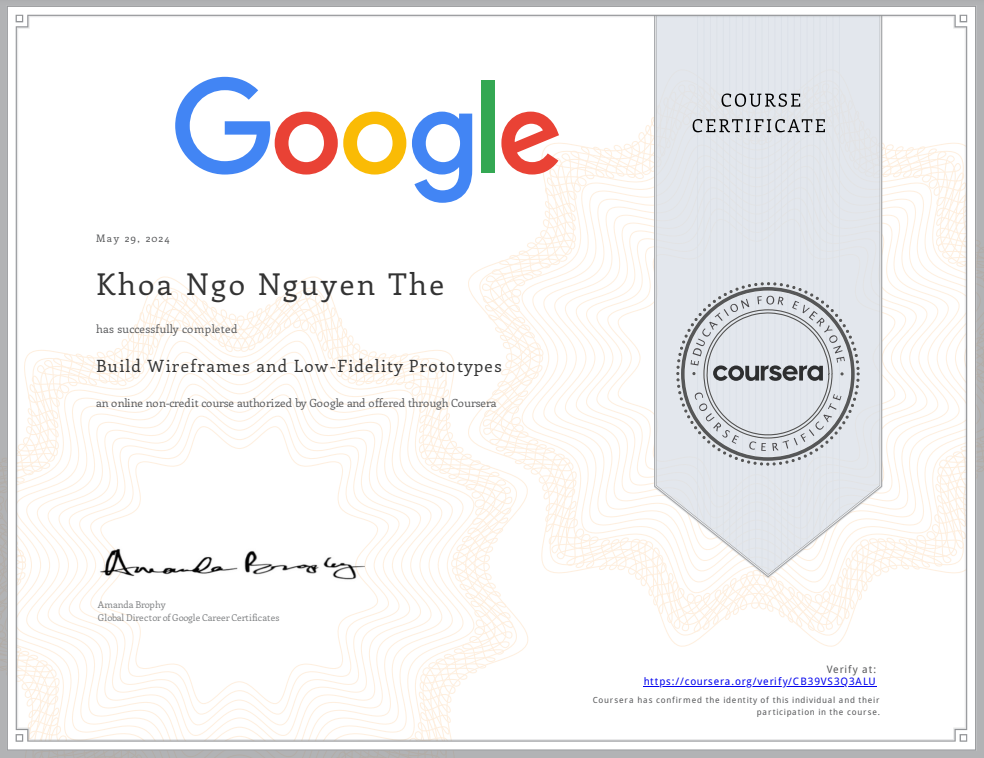
\includegraphics[width=0.85\textwidth]{imgs/Course3.png}
		\caption{Course 3 Certificate}
	\end{figure}

	Visit the online certificate for more info \href{https://www.coursera.org/account/accomplishments/verify/CB39VS3Q3ALU}{here}
\end{flushleft}

\subsubsection{Summary}
\begin{flushleft}
	What I have learned after completing this course:
	\begin{itemize}
		\item Create storyboards to come up with ideas about solutions to user needs.
		\item Create wireframes on paper and digitally in the design tool Figma.
		\item Build paper prototypes to create interactive designs.
		\item Design low-fidelity prototypes in Figma.
	\end{itemize}
\end{flushleft}

\subsubsection{Details}
\begin{flushleft}
	\begin{description}
		\item[Module 1:] Storyboarding and wireframing
		      \begin{itemize}
			      \item I have learnt how to use research findings to inform ideation during the design process.
			      \item I have created two types of storyboards: big picture and close-up.
			      \item I have drawn my first wireframes, and explored the benefits of wireframing.
		      \end{itemize}
		\item[Module 2:] Creating paper and digital wireframes
		      \begin{itemize}
			      \item I have learnt Figma about how to best use their tool.
			      \item I have applied Gestalt Principles, like similarity, proximity, and common region, to my wireframes.
		      \end{itemize}
		\item[Module 3:] Building low-fidelity prototypes
		      \begin{itemize}
			      \item I have transition to a digital low-fidelity prototype in Figma.
			      \item I have explored ways to recognize potential bias in my designs and learnt how to avoid deceptive patterns.
		      \end{itemize}
	\end{description}
\end{flushleft}